\documentclass[midd]{thesis}

\usepackage{graphicx}
\usepackage{times}
\usepackage{amsmath}
\usepackage{booktabs}
\usepackage{lscape}
\usepackage[table,xcdraw]{xcolor}
\usepackage{listings}
\usepackage{color}



\bibliographystyle{plain}
\title {Computational Aesthetic Evaluation using Convolutional Neural Networks}
\author {Edward Knox}
\adviser {Professor Christopher Andrews}

\begin{document}
\maketitle









\begin{abstract}
State-of-the-art machine learning techniques have become competitive with humans at certain limited tasks, suggesting that computers will soon play a role in tasks traditionally completed by humans alone. One such field is computational aesthetics which aims to train computers to recognize beauty through an understanding of human aesthetic judgements. This study tested the accuracy of a state-of-the-art convolutional neural network for modeling the user-defined visual aesthetic tastes on randomly generated triangle art. Our trained model demonstrates a modest accuracy above ``random'' of 2.9\%, suggesting that more work lies ahead in understanding how pattern recognition fits into the puzzle of computational aesthetic evaluation.
\end{abstract}

\begin{acknowledgements}
I'd like to thank Professor Andrews for his patience and wisdom in guiding my newfangled exploration of the world of academic research. 
\end{acknowledgements}

\contentspage
\tablelistpage
\figurelistpage

\normalspacing \setcounter{page}{1} \pagenumbering{arabic}
















\chapter{Introduction}
\label{sec:intro}

% TODO: Cite better than human performance from machine learning

% general introduction to CAE and generative art
% why we would care? vision
% WHat is this particular thesis about -> applying ml to the problem
% what are we doing? -> convolutional neural network
% more specific -> ran a study, using GoogLeNet
% What we will discuss ->

Machine learning is a broad discipline of computer science that has seen rapid advances in recent years, and has the potential to impact all human enterprises. The latest algorithms are capable of competitive or better-than-human performance on certain tasks, and their applications are increasing the availability of training data. One such application will be in the field of generative art and design. Generative art is art that is created procedurally, with the help of a computer. Until recently, the use of computers in art and design had been limited to rote tasks such as preparing renderings and generating randomness, but advances in machine learning may soon enable computers to contribute to higher-level aspects of the creative process, such as strategic planning and aesthetic evaluation. Computational aesthetics is a subfield of generative art research concerned with training a computer to subjectively differentiate between aesthetically pleasing and displeasing content. Within the field of generative art, this problem is integral to the task of automating searches for aesthetic solutions, and further personalizing recommendation systems. This research investigates the applicability of state-of-the-art general-purpose pattern recognition algorithms to computational aesthetic evaluation. This experiment is motivated by an interest in discovering the limits of these impressive models. By evaluating their accuracy on unconventional datasets of unknown complexity, we hope to gain a better understanding of both the model's capabilities and the underlying predictive structure of the data. This paper first provides background, then formulates the problem, then explains the experiment in detail, and finally concludes with a discussion of results and ideas for future research in computational aesthetics.

Convolutional Neural Networks (CNNs) are a type of model inspired by the biology of the human visual processing center, and have been shown to be the most effective model for image recognition to date.
% TODO: Cite this assertion
CNNs are a type of feed-forward artificial neural network architecture formed by layers of convolutional filters, trained to derive high-level features from low-level pixel data. These high-level features are powerful and versatitle data separators which are typically fed into a non-linear classifier or regressor to produce predictions. The network's parameters are learned through an iterative training process, where the model is tested on batches of examples, and network parameters are adjusted to correct for prediction errors. Iterations of adjustments are made until the network's prediction accuracy on the test dataset converges or shows signs of overfitting.
























\chapter{Background}
Before discussing the particulars of this study, we will first explain background principles motivating our interest in the fields of Computational Aesthetics and Image Recognition.

\section{Computational Aesthetics}
Computational aesthetics is a fledgeling interdisciplinary field formed by the overlap of research in machine learning, neuroethetics, and evolutionary psychology. Efforts in this field have been mostly explorational, as few concrete advances have been made. Some of the most-cited papers in the field of Computational Aesthetics are titled ``Computational aesthetic evaluation: Past and future'', ``Defining computational aesthetics'', and ``Experiments in computational aesthetics'', indicating on a high level the field's stage of development. These studies fall into practical and theoretical categories, roughly corresponding to top-down and bottom-up research strategies. Practical studies tend to be oriented around conducting experiments to verify the correlation of commonly-held aesthetic heuristics with subjective aesthetic ratings, in effect studying the correspondences of these guidelines and true aesthetic ratings. Theoretical studies aim to develop a connectionist model for understanding aesthetics by drawing upon the insights of machine learning and neuroaethetics, in the hope of making new generalizations on the nature of aesthetics \cite{galanter2012computational, hoenig2005defining, machado2008experiments}.

% TODO: Talk about top-down work

Top-down work in computational aesthetics aims to develop an enlightened philosophical framework for understanding the human aesthetic system, and is indispensible for thinking clearly about bottom-up experimental work. Galanter and Hoenig grapple head-on with the field's conceptual entanglement, with an awareness of the ``baby steps'' necessary before significant advances. We suspect, and we think these researchers would agree, that generalizable advances in this field will be more deeply related to machine learning and neuroesthetics (the study of aesthetics from a biological perspective), rather than more pragmatic areas of aesthetics, such as the study of Gestalt laws. Given that philosophers have been devising high-level heuristics for judging aesthetics since antiquity, it seems unlikely that the increased availability of computational power will directly impact our conception of this problem.

To provide further context, we will briefly summarize the history of computational aesthetics and survey research strategies within the field.

\subsection{Philosophical Underpinnings Computational Aesthetics}

One of the first significant advances in the greater philosophy of aesthetics is owed to Mathematician G.D. Birkoff, who spent a year traveling the world to study beauty across cultures, before proposing a speculative psychological model for quantifying it. In his oft-referenced 1933 paper \emph{Aesthetic Measure}, Birkoff proposes that the perception of beauty is the pleasurable resolution of apparent complexity of a stimulus into a compact mental representation. He codified this relationship into a formula that relates the degree of beauty $B$ to the balanced ratio of order $O$ to complexity $C$.

\begin{align*}
B &= \frac{O}{C}
\end{align*}

The plausibility of Birkoff's measure as a guiding philosophy of aesthetics earned it significant attention in later experimental studies. The recent work of Ragau et. al. and Koshel et. al. draws from information theory to approximate the parameters of Birkoff's formula. They used zeroth-order measures such as Kolmogorov complexity and Shannon entropy \cite{rigau-1, koshelev-1}, to demonstrate encouraging correlations between Birkoff's measure and human-rated beauty.

These results are significant enough to validate the direction Birkoff's core idea --- that the human aesthetic response is tuned to respond to stimuli that are both sophisticated and digestible. Novel ideas in the fields of machine learning, neuroesthetics, and the emerging field of evolutionary philosophy (the top-down study of evolutionary adaptations), may be a way forward.
% TODO: rework the following
Philip Galanter stands at the intersection of these fields, and subscribes to the view that humans find stimuli with the greatest ``effective complexity'' to be the most engaging, and thus the most rewarding. Within this framework, the problem of computational aesthetics can be expressed as the study of how humans judge ``effective complexity'' \cite{galanter-1,galanter-2,galanter-3,galanter-4}. Effective complexity is a theoretical measure conceived by Gell-Man et. al. \cite{gell2004effective} to roughly correspond to the colloquial meaning of the word ``complex''. Effective complexity measures resistance to entropic forces rather than resistance to signal compression. For example, a symphony by Mozart possesses greater effective complexity than white noise, because it presents a manageable amount of harmonious sophistication for most people to process.

\begin{figure}
\centering
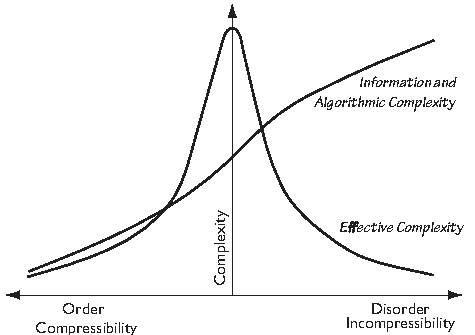
\includegraphics[width=0.75\textwidth]{figures/effectivecomplexity.pdf}
\caption{Relationship between effective complexity and order}
\label{fig:effectivecomplexity}
\end{figure}

In seeking to develop a computational aesthetic evaluator this research touches onto topics of information complexity and effective complexity, as developed by these researchers. These improving conceptual measures will likely align closely with the theory underlying the neurology of human sensory perception. It may already be possible to draw parallels between the principles underlying machine learning systems and Birkoff's measure, since the success of these systems already depend on the learning of compact, high-level represenations of low-level inputs. This is one of the reasons we became interested in applying the latest advances in image recognition to the field of computational aesthetics. The discovery of convolution-like neural structures in the visual cortex of the brain leads us to speculate that convolutional neural networks may demonstrate predictive power in evaluating aesthetics.


\subsection{Survey of Experiments in Computational Aesthetics}

Experimental progress in computational aesthetic evalution has tended to ride the coattails of advances in the machine learning, albiet with some lag, and thus advances have come slowly but steadily. The curve of advances has only seen two high-level stages. Early studies in this field tended to rely on heuristic-based feature-extractors, and more recent studies have moved towards the use of learned feature hierarchies to make independent generalizations from raw data.

\subsubsection{Models Relying on Heuristic Measures as Features}

% TODO: Find the real study

The low-hanging fruit of computational aesthetic evaluation (CAE) algorithms are those which incorporate commonly held aesthetic heuristics, such as the rule of thirds, into supervised shallow machine learning classifiers to make predictions on simple datasets. The main goal of experiments involving these algorithms tends to be investigating how predictive these heuristics really are, or to test the applications of these algorithms.

One experiment of this kind aimed to model user ratings of photographs sourced from an online photography community based on their aesthetic value. Zhou et. al. used a decision tree and numerical measures of symmetry, aspect ratio, adherence to the rule of thirds, etc. to do so \cite{zhou2014computational}. Their model achieved a 70\% classification accuracy, which is impressive considering there was no specialized image recognition technology involved in the experiment. Simple models like these demonstrate that in certain situations, relatively simple machine learning techniques can do much better than random at aesethetic evaluation. These results are encouraging, but it is important to take into consideration the quality and limited scope of this dataset. Within a vacuum, it may be possible to manually develop predictive features for a particular dataset, but this approach is labor intensive and misses out on predictive features not manually mined.

% TODO: Replace useless study description
Penousal Machado et al \cite{machado2008experiments} implemented an iterative artificial artist system by combining a neural network with an evolutionary programming system. The neural network served as an aesthetic evaluator, and was trained on manually extracted features for every step of the iteration. The genetic programming system would generate populations of artwork and use the aesthetic evaluator as its fitness function. In observing the creative process as a series of alternations between creative and evaluative stages, their system repeatedly produces populations of ``drafts'' and then evaluates how well they match a constant set of target images of painterly artwork. The drafts that most closely matched the target images would then seed the next generation of drafts, and the aesthetic evaluator would be retrained to recognize all of the drafts as non-target images. This feedback loop was designed to incentivize every generation of drafts to be different from the last, hopefully resulting in greater image complexity. The entire algorithm produces interesting results until the 12th generation, when classification error increases too steeply to encourage any more variation.

The system's aesthetic evaluator uses 41 features based on metrics like fractal complexity and zipf distribution, each applied over a variety of image channels such as hue or saturation. Although these features provided some predictive value, none were discovered to be orders of magnitude more predictive than the others. This experiment demonstrates how neural networks are being applied in novel ways to explore computer capabilities for generating and recognizing aesthetically pleasing art. % maybe cut this out?

Many have also put genetic algorithms to the task of coming up with novel solutions to design problems, and have incorporated aesthetic features into their fitness function by manually extracting heuristic measures. These approaches demonstrate acceptable results, and are generally limited by their set of handmade low-level features for prediction. % citations??

\subsubsection{Models Using Learned Feature Extraction}

The future of computational aesthetics is tied to the future of machine learning, and future of machine learning involves onloading more and more of the feature extraction process to trained feature extractors, so that those features with the greatest predictive power can be found algorithmically rather than by trial and error. Several studies of computational aesthetic evaluation have begun investigating the applicability of ``deep'' learning algorithms for greater generalization and accuracy in computational aesthetic evaluation. 

In one such study, Allan Campbell used self-organizing maps, a type of neural network inspired by structures in the brain's auditory cortex, as a way to identify features of images with high relevance to abstract image aesthetics \cite{campbell2013self}. His work was successful in identifying several low level features such as ``image smoothness at scales'' as important in human evaluation of aesthetics, and also demonstrates the applicability of self-organizing maps for CAE.

This study looks into the applicability of a different kind of ``deep'' learning algorithm called convoluational neural networks, which builds deep representations of images through supervised training, and classifies those representations using a standard fully-connected neural network. Only a few studies have looked into the properties of these powerful and tested algorithms in relation to computational aesthetics.

One relevent study performed by Lake et. al. looked at whether human typicality ratings of images correlate with the classification confidence of a convolutional neural network \cite{lakedeep}. Typicality, possibly short for prototypicality, is a psychological measure of how closely a given example conforms to a person's idealized image of its kind. For example, in the study, users were shown images of towels and asked to rate how ``towel-like'' the towel appeared. Galanter speculates that prototypicality plays an important role in human aesthetic judgements, so computer performance on task of this kind are likely relevant to CAE \cite{galanter-4}. Lake et. al. used several architectures of convolutional neural networks, including GoogLeNet, to measure the correlation between user ratings of image typicalities and the model's confidence in classifying that object. They discovered significant correlations, and the magnitudes of these correlations seemed proportional to the accuracy of the classifier used. The relationship between typicality ratings and aesthetics, and between GoogLeNet's prediction confidence and typicality ratings strongly suggest that further study of CNNs is likely to be fruitful.





















\section{Related Work in Image Classification}

Image recognition techniques within the field of machine learning present some of the most promising opportunities for advances in computational aesthetics. The accuracy and prevalence of state-of-the-art pattern recognizers have been increasing steadily for the last decade. Leading researchers claim that these encouraging advances in data science have been the result of a combination of the increasing availability of huge datasets, the decreasing cost of computation, and the influx of new ideas \cite{szegedy2014going}. As the field has grown, so has the availability of user-friendly frameworks for implementing machine learning architectures, allowing for greater interdisciplinary use of these models.


Although many strategies exist for constructing image recognition models, by far the most effective strategy in recent years has been the ``convolutional neural network'', a specific architecture of neural network that makes use of hierarchical convolutional filters. Convolutional Neural Networks date back to 1989, when Yann LeCun demonstrated their efficacy at classifying simple images of digits\cite{lecun1989generalization}. A year later, his ``LeNet'' classified a real-world image dataset of handwritten postal code digits with impressive accuracy \cite{Cun90handwrittendigit}. Decades later, CNNs became widely recognized as one of the most powerful architectures when Krizhevsky et. al. \cite{NIPS2012_4824} handily won the ImageNet ILSVRC 2012 competition, using a massive CNN architecture. The 2012 Imagenet Large Scale Visual Recognition Challenge provided competitors with 1.2 million labeled images, challenging models to discriminate between 1000 image classes, and was the most difficult object categorization benchmark at the time. The winning submission, dubbed ``AlexNet'', made 40\% fewer errors than the next best competitor, sporting 84.7\% acccuracy. Needless to say, submissions to the 2013 ILSVRC competition were all variations of CNNs. The 2014 ILSVRC was won by the research team at Google with a CNN nearly $3\times$ deeper and with $12\times$ sparser than AlexNet. The accuracy of GoogLeNet was 94.4\%. GoogLeNet's ability has likely been superceded by another variation of CNN by now, but for the purposes of this study it suffices to label this model as state-of-the-art.

Convolutional neural networks are defined by their ability to produce abstract high-level representations of raw low-level inputs, using a hierarchy of shared-weight convolutional filters implemented with neural networks. LeCun conceived of convolutional neural networks during a time when fully-connected neural networks were an area of intense study. The same year LeCun published his paper, Cybenko published a landmark proof showing that neural networks were universal function approximators \cite{cybenko1989approximation}. 

\begin{figure}[h]
\centering
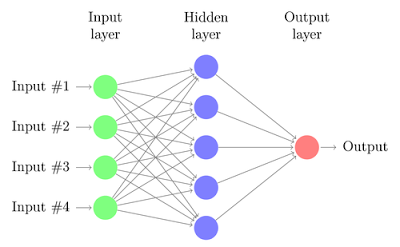
\includegraphics[width=\textwidth]{visualizations/nn.png}
\caption{Visualization of a two-layer fully-connected neural network}
\label{fig:nn}
\end{figure}

One of the drawbacks of fully-connected neural networks is their tendency to overfit the data, causing an unpredictable loss in generalization performance across datasets. LeCun attributed this to their complete lack of \emph{a priori} parameterization with which to make necessary assumptions about the data's distribution. Another recognized problem with fully-connected neural networks is the difficulty of training more than a few layers of neurons without encountering the problem of ``vanishing gradients'', where the backpropagation algorithm cannot effectively train low-level layers because error gradients fall to zero too quickly. 
% curse of dimensionality?
LeCun's architecture addressed these issues by dramatically reducing the parameters (connections) in his multi-layered neural network without greatly significantly reducing its classification power. Inspired by prior image recognition advances, he adapted filter hierarchies to the structure of neural networks to build high-level abstractions without running into the problems mentioned above. 

The core conceptual unit of this idea is the convolutional filter, which can be thought of a small, square image patch that is run over every compatible region in the 2D input vector. At each location on the input, the overall degree of similarity between the filter and the overlapping region of the input is calculated using an inner-product calculation, and then assigned as the output value for that pixel on the 2D output vector. After the filter intensity is calculated for specific output location, that intensity value is fed through a sigmoidal activation function to supress smaller activations. This decision is made under the observation of the same assumption guiding fully-connected NNs, which is that small activations are disproportionally less predictive than large activations within the current scheme. Each convolutional filter produces its own 2D output vector. 

\begin{figure}[t]
\centering
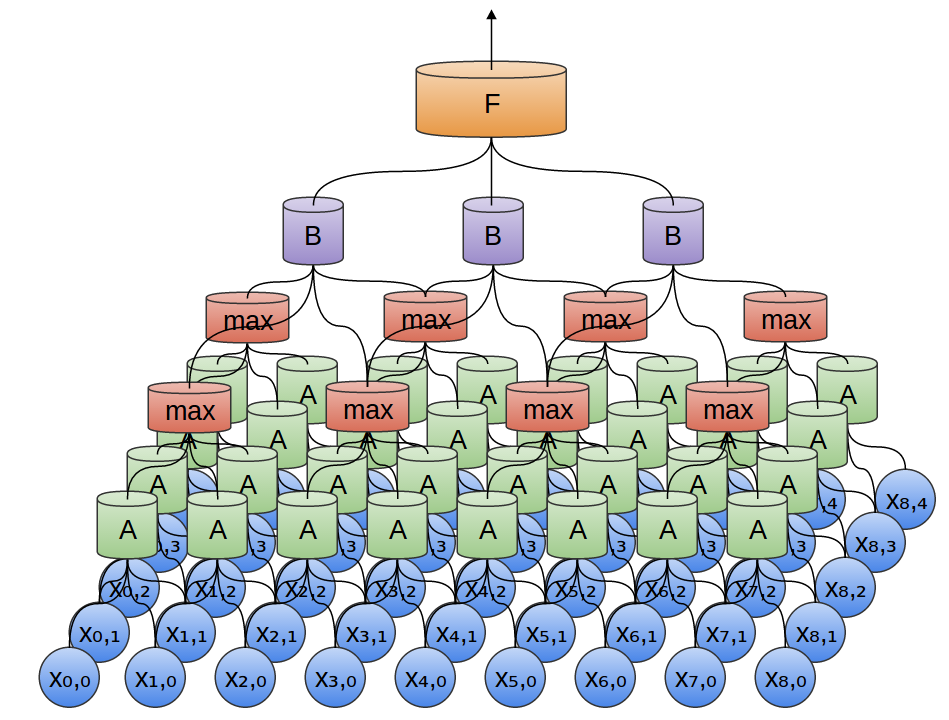
\includegraphics[width=0.5\textwidth]{visualizations/simple-cnn.png}
\caption{Simple CNN with 2 convolutional layers, one filter each.}
\label{fig:cnn-in-neurons}
\end{figure}

In implementing a convolutional filter using neurons, a single convolutional filter of size $R\times R$ over an input vector of size $N\times N$ roughly corresponds to a set of $N^2$ neurons sharing a single set of $R^2$ weights over roughly $N^2R^2$ connections. The shared weights vector represents the pixel intensities of the filter. To formalize this idea, LeCun invented the concept of sharing network parameters between connections, so that each filter would be applied the same across the entire input vector.

In designing large-scale convolutional neural network, many ``layers'' of feed-forward filter ``banks'' are wired together, and often finally connected to a shallow fully-connected network to produce classification outputs. A filter bank is a set of filters within a single layer. Between layers, the output from every filter is wired up as input to every filter in the next layer, and so to avoid a combinatorial explosion of training weights, layers are typically separated by dimensionality-reducing and regularizing filters.

\begin{figure}[h]
\centering
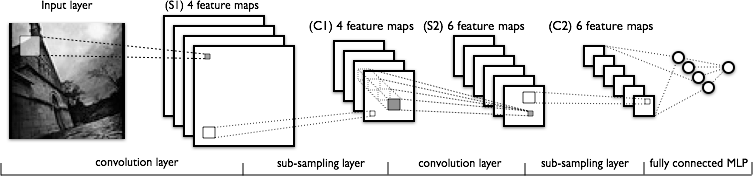
\includegraphics[width=0.5\textwidth]{visualizations/Mylenet.png}
\caption{Visualization of the architecture of a CNN.}
\label{fig:mylenet}
\end{figure}

The training of convolutional neural networks follows the same process as feed-forward networks. A loss function guides a batch gradient descent algorithm, which iteratively updates network weights by backpropagating the network's inverted error gradient for classifying that batch.























\chapter{Design}

Three motivations informed the design of this experiment.

The first was an interest in whether convolutional neural networks might prove more effective than hand-programmed feature extractors for computational aesthetic evaluation. In our literature review we noticed that a majority of experiments in aesthetic evaluation rely on tens of hand-programmed feature extractors and standard machine learning classifiers to produce decent results. These approaches are based on rigid assumptions on the manifestations of aesthetic value. One of these experiment extracted a feature corresponding to the dynamic contrast of colors in the image, and another feature corresponding to the diversity of colors in an image patch. Using a bunch of hand-programmed feature extractors in these experiments is one way to search for ultra-effective feature extractor, but if this search is not fruitful it may make sense to turn towards more versatile feature extraction techniques. In the task of image recognition, convolutional neural networks are effective for recognizing extremely different patterns; could a CNN do for aesthetic evaluation what it did for image recognition?

The second motivation informing the design of this study was an interest in the separability of subjective aesthetic judgements of arbitrary complexity. We wanted to throw a dataset of unknown difficulty at our model and see how it would perform. There is much hype surrounding the capabilities of this type of model, some of which we admittedly bought into. In an effort to challenge our expectations of these models, we asked whether such a model could demonstrate effectiveness on a dataset it was not designed for. To do this, the ratings forming our dataset were sourced from a single user to impart an esoteric and personal quality to the dataset, and to experiment with new machine learning methods for recommendation systems.

The third motivation was an interest in the relationship between the accuracy of our classifier for a given image and the type of image provided to the classifier. If we used a simple type of art for our experiment, it might be easier to identify patterns in the characteristics of images that the classifier found it difficult and easy to classify.

With these factors in mind, we designed an experiment. The body of artwork for rating would be randomly generated triangle art. We would build a training interface for rating these images, where for each rating the user would assign the presented image a completely subjective binary rating of attractiveness. Clicking the green button would mark an image as good-looking, and the red button would mark it otherwise. In order to ensure the internal consistency of ourratings, we would make sure the user rated each image more than once rating during the training proces. We represented positive ratings as 1s, and a negative ratings with 0s. If an image received conflicting ratings, its recorded label would cast to 1, to bias our classifier towards false positives rather over false negatives.

To perform this experiment we would need to assemble a relatively small dataset of images labeled ratings using a training interface, and we would need an instance of the GoogLeNet classifier. To assess the accuracy of our model over this small dataset we would perform the commonly-used 10-folds cross-validation technique and judge performance by averaging over the best performing model iteration for each fold.























\chapter{Implementation}
\section{Training Interface}

Assembling a dataset was relatively straightforward. We built an interface for generating images and recording their user ratings using python and web technologies. After each rating submission, the interface algorithmically decided which image to show next. We programmed to randomly alternate between presenting new images and existing images, with a bias towards presenting those existing images with the fewest ratings.
% TODO: Flagged for removal
For convenience, we added swipe gesture support to the mobile interface, allowing for rating on-the-go.
% TODO: Image of mobile interface

Our algorithm for generating an image worked as follows. First a blank $256\times 256$ canvas would be filled with a random color. Then a random number of triangles (between 2 and 6) would be drawn on top of each other. Triangles' corners would be randomly placed, and their fill color would be random. All of the randomness used was uniform, and all of the colors were specified in HSL format, so that the lightness of each randomly-selected color could be restricted to an attractive range of values.

% TODO: Position xkcd graphic connoisseur.png https://xkcd.com/915/
\begin{figure}
\centering
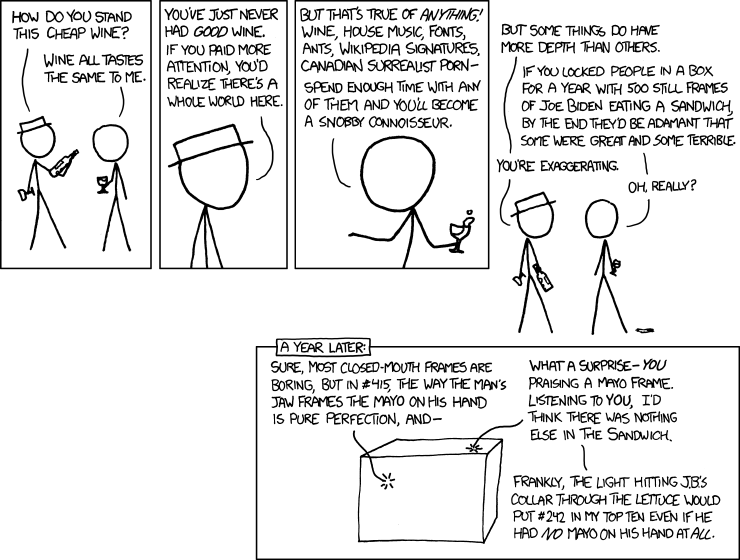
\includegraphics[width=0.9\textwidth]{visualizations/connoisseur.png}
\caption{Relevant xkcd: Aesthetic judgements can be arbitrarily esoteric.}
\label{fig:effectivecomplexity}
\end{figure}

Over the course of a few days the user made roughly 4000 ratings of 2000 images. In rating triangle art for several hours the user quickly would grow tired of making aesthetic judgements of images. Within the literature of computational aesthetic evaluation this is referred to as ``user fatigue'', and is a recognized impediment to the training of intelligent interactive systems, as it dramatically limits the scale of data collection for an individual. In order to reach 4000 high-quality ratings, we found it useful to suggest that the user take breaks, and also urged him to resist any drift in aesthetic judgements based on novelty (although novelty certainly factors into aesthetics). Our decision to stop at 4000 ratings was rather unscientific, though guided by intuition. At this stage in the experiment we became anxious to begin working with our data, and we felt a dataset of, say, 10,000 examples would not be significantly better than a dataset of 4,000 examples. 

\begin{figure}
\centering

\includegraphics[width=0.9\textwidth]{visualizations/sample-random.png}
\caption{Examples of the generative art we rated. Our user gave the image in the top right a postive rating.}
\label{fig:effectivecomplexity}
\end{figure}

% dataset size by model accuracy
This intuition was based on the published results of tech companies using large datasets to tackle hard problems like language translation and image captioning. Unless we could produce at least an order of magnitude more training examples, we supposed that the accuracy of our resulting model would not vary by much. Once converting image scores to labels, 73.3\% of the images were labeled as having low aesthetic value and the remaining 26.6\% with high aesthetic value.
% TODO: verify priors
\begin{table}[h]
\centering
\begin{tabular}{@{}cc@{}}
\toprule
\multicolumn{1}{l}{Label} & \multicolumn{1}{l}{Quantity} \\ \midrule
0 & 1707 \\
1 & 646 \\ \bottomrule
\end{tabular}
\caption{Distribution of image labels}
\label{score-distribution}
\end{table}
% TODO: sigmoid graph of data quantity by model accuracy

\section{Classifier}

We decided to use a popular neural network modeling framework called ``Caffe'' to implement our classifer. Caffe began at the Berkeley Language and Vision Center in 2013, and offers a well-designed and efficient interface for designing, training, and running neural networks. Caffe comes packaged with several example model specifications, one of which thoroughly describes an untrained replica of GoogLeNet. Using this specification ensured the accuracy of our model, and was utterly convenient.

\begin{figure}[h]
\centering
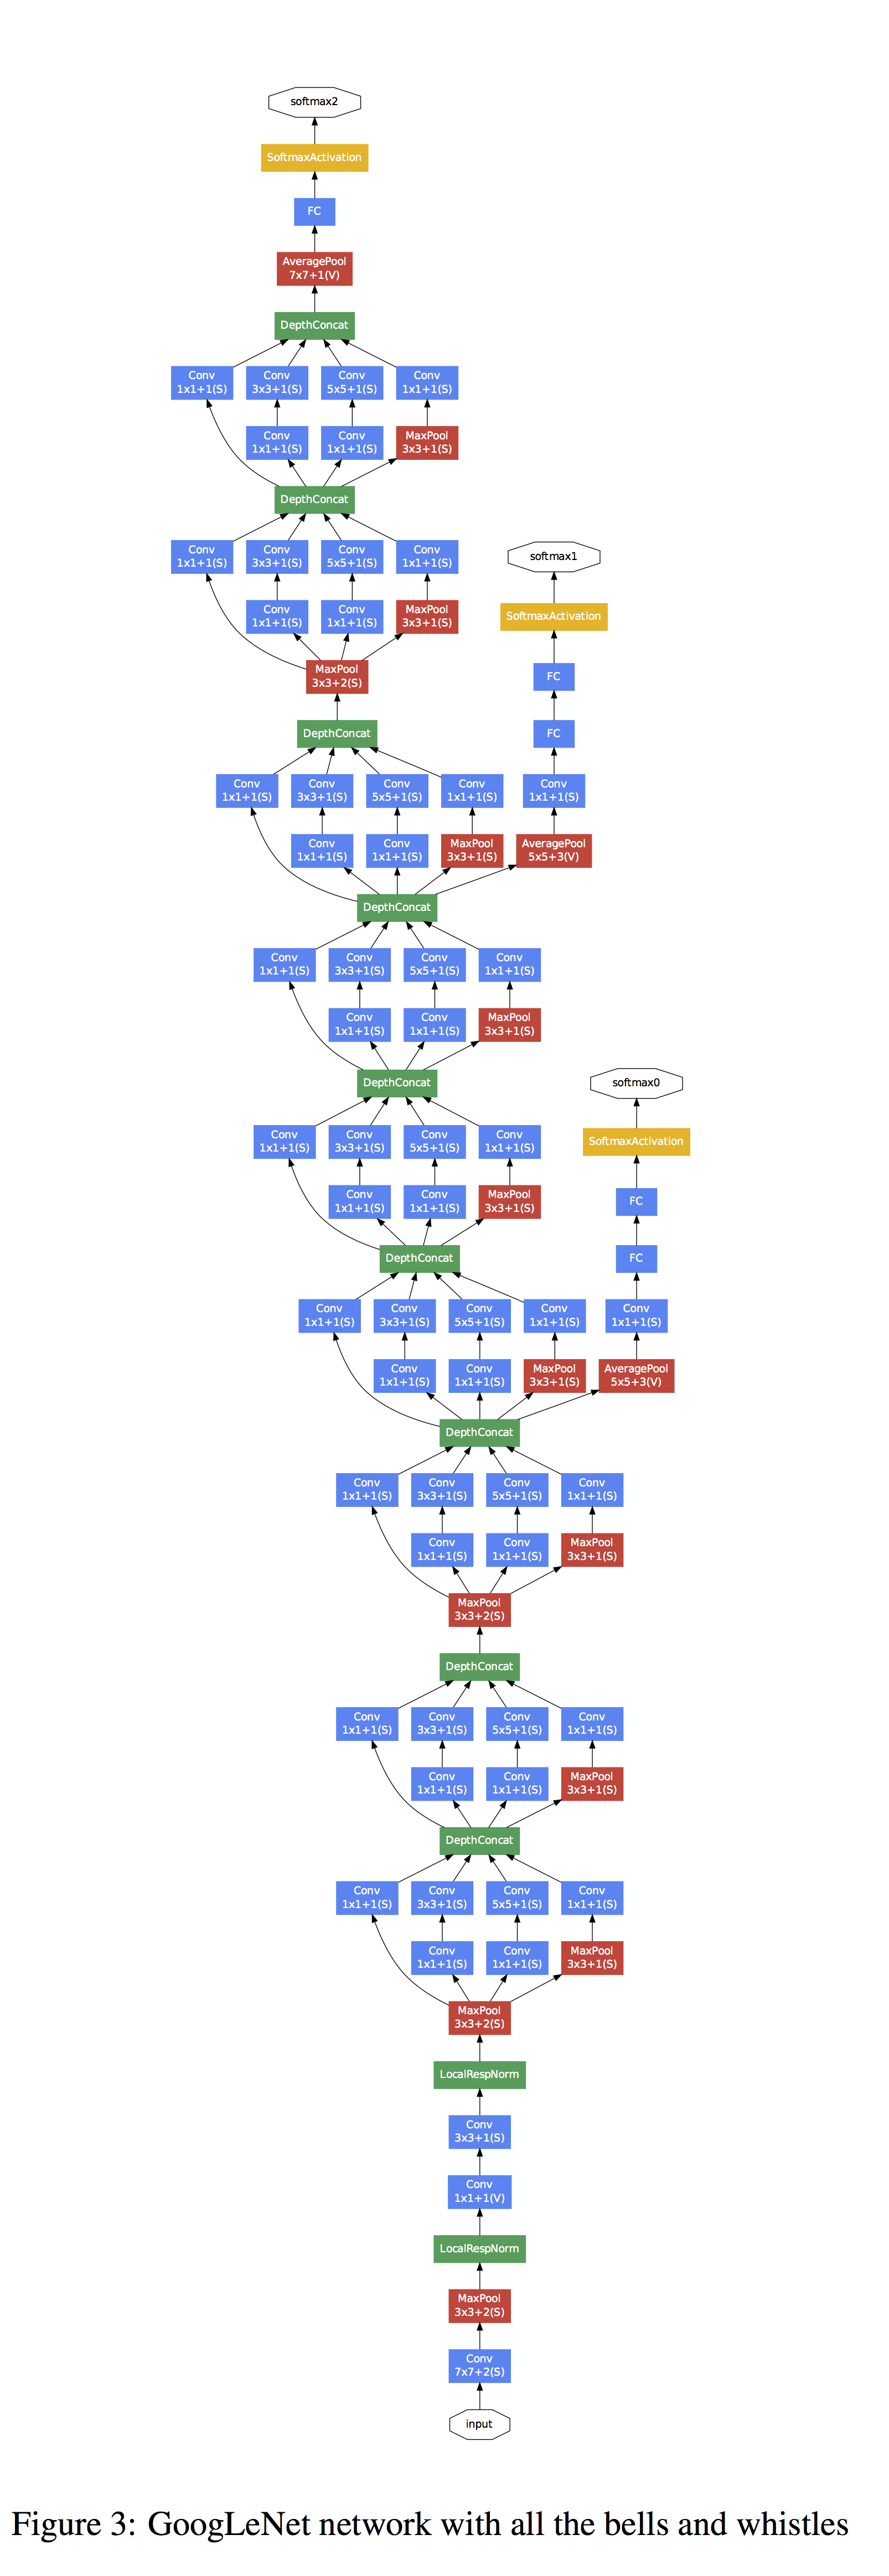
\includegraphics[width=0.9\textwidth]{figures/googlenet.png}
\caption{Flow chart representing GoogLeNet's layers.}
\label{fig:googlenet}
\end{figure}

The convolutional neural network training process is computationally intentensive, requiring training time that grows quickly with the width and number of layers. GoogLeNet is a large, 22-layer CNN that would requires significant resources to run. To model our data in a resonable amount of time, we decided to rent an Amazon g2.2xlarge cloud instance, complete with a graphics card sporting 1,536 CUDA cores. This allowed for us to take advantage of enticing GPU speedups that Caffe optionally offers.\footnote{This cloud setup was convenient both financial and technically. Amazon's pay-as-you-go billing model meant we only paid for computing resources that we used, and their transparent cloud imaging technology meant that our Caffe installation persisted through restarts. Instant remote access to high-powered computing is a magical experience.}
% TODO: CPU VS GPU graphic

\begin{figure}[h]
\centering
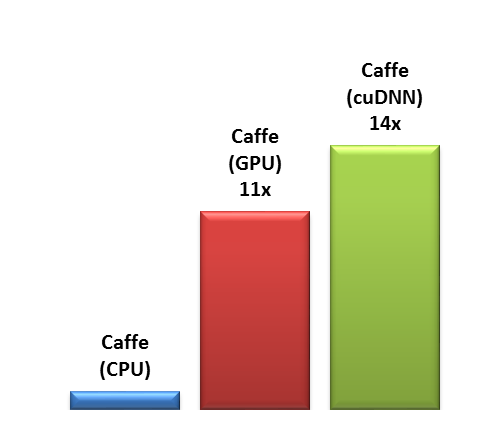
\includegraphics[width=0.5\textwidth]{visualizations/caffe-performance.png}
\caption{Caffe performance benchmark acrosss installation types (higher is better).}
\label{fig:caffebenchmark}
\end{figure}


Next we retrofitted the provided GoogLeNet architecture to produce predictions for 2 labels, instead of 1000. Finally we wrote bash scripts to automate all 10 folds of the experiment's execution, which included data splitting, data preprocessing, model training, model testing, and log parsing, and statistical aggregation.






















\chapter{Results}
% \begin{landscape}
\begin{table}[h]
\centering
\resizebox{\textwidth}{!}{%
\begin{tabular}{@{}rlllllllllllll@{}}
\toprule
\textbf{k-Fold} & \multicolumn{10}{c}{\textbf{Training Iteration}} & \textbf{\begin{tabular}[c]{@{}l@{}}Best \\ Accuracy\end{tabular}} & \textbf{\begin{tabular}[c]{@{}l@{}}Null\\ Hypothesis\\ Accuracy\end{tabular}} & \textbf{\begin{tabular}[c]{@{}l@{}}Accuracy\\ Above \\ Null\end{tabular}} \\ \midrule
\textbf{} & 100 & 200 & 300 & 400 & 500 & 600 & 700 & 800 & 900 & 1000 &  &  &  \\ \midrule
\multicolumn{1}{r|}{1} & 0.758 & 0.766 & 0.756 & 0.766 & \textbf{0.781} & 0.768 & 0.773 & 0.770 & 0.770 & \multicolumn{1}{l|}{0.773} & 0.781 & 0.765 & 0.016 \\
\multicolumn{1}{r|}{2} & 0.705 & 0.699 & 0.715 & 0.715 & 0.732 & 0.727 & \textbf{0.746} & 0.734 & 0.732 & \multicolumn{1}{l|}{0.707} & 0.746 & 0.738 & 0.027 \\
\multicolumn{1}{r|}{3} & 0.754 & 0.765 & 0.758 & \textbf{0.803} & 0.748 & 0.691 & 0.752 & 0.682 & 0.767 & \multicolumn{1}{l|}{0.723} & 0.803 & 0.761 & 0.042 \\
\multicolumn{1}{r|}{4} & 0.752 & 0.752 & \textbf{0.770} & 0.762 & 0.738 & 0.75 & 0.760 & 0.756 & 0.752 & \multicolumn{1}{l|}{0.756} & 0.770 & 0.755 & 0.014 \\
\multicolumn{1}{r|}{5} & 0.695 & 0.707 & 0.676 & 0.707 & 0.682 & 0.709 & 0.697 & \textbf{0.713} & 0.709 & \multicolumn{1}{l|}{0.699} & 0.713 & 0.699 & 0.014 \\
\multicolumn{1}{r|}{6} & 0.709 & 0.713 & 0.736 & 0.707 & 0.725 & 0.699 & 0.738 & \textbf{0.748} & 0.734 & \multicolumn{1}{l|}{0.713} & 0.748 & 0.713 & 0.035 \\
\multicolumn{1}{r|}{7} & 0.699 & 0.699 & \textbf{0.752} & 0.723 & 0.699 & 0.729 & 0.699 & 0.727 & 0.717 & \multicolumn{1}{l|}{0.707} & 0.752 & 0.700 & 0.052 \\
\multicolumn{1}{r|}{8} & 0.764 & 0.760 & 0.766 & 0.758 & 0.768 & 0.773 & 0.766 & 0.750 & 0.758 & \multicolumn{1}{l|}{\textbf{0.797}} & 0.797 & 0.757 & 0.039 \\
\multicolumn{1}{r|}{9} & 0.703 & 0.715 & 0.658 & 0.707 & 0.684 & \textbf{0.714} & 0.713 & 0.705 & 0.709 & \multicolumn{1}{l|}{0.697} & 0.714 & 0.699 & 0.016 \\
\multicolumn{1}{r|}{10} & 0.740 & 0.748 & 0.742 & 0.729 & 0.736 & 0.752 & \textbf{0.766} & 0.760 & 0.727 & \multicolumn{1}{l|}{0.764} & 0.766 & 0.738 & 0.027 \\ \midrule
\multicolumn{1}{l}{\textbf{}} &  &  &  &  &  &  &  & \multicolumn{3}{r|}{\textbf{Average}} & 0.762 & 0.733 & 0.029 \\ \bottomrule
\end{tabular}
}
\caption{GoogLeNet test accuracy across 10-fold cross-validation and compared with null hypothesis priors}
\label{results}
\end{table}
% \end{landscape}

% TODO: Verify priors
On average, our model demonstrated a classification accuracy of 0.762\%, only 2.9\% greater than the accuracy of the null hypothesis model. \footnote{The null hypothesis model is the fake classification model that always predicts the class with the greatest prior probablity of occurence. In this experiment, the average prior probability of encountering an low aesthetic image was 73.3\%, meaning that the null hypothesis model would be this same accuracy by always predicting low aesthetic.} Although this result does not suggest that our model was adept at predicting labels for this dataset, its slight increase over random leaves the door open to further exploration, perhaps backed with more theory.

It has been said in the machine learning that the optimization of hyperparameters is at times more art that science, and this aphorism certainly applies to our experiment. Our initial training runs lead to instances of gross overfitting, leading us to discover that several of the default stochastic gradient descent parameters for training GoogLeNet would not be appropriate in our case. 

The combination of a paucity of data and a massive model made for extremely fast convergence to our best results. For comparison, our model would train to its best test accuracy within 1000 training iterations, while it was not unusual for Google Research to train GoogLeNet for upwards of 2,400,000 iterations on ILSVRC competition data. Our model tended to bounce around its test accuracy optimum even using a small step size, indicating that increases in accuracy on the training set almost immediately stopped translating into increases in accuracy on the test set. Unfortunately this accuracy of this result does not provide us with enough information to draw concrete conclusions about the applicability of convolutional neural networks for visual computational aesthetics tasks. The ineffectiveness of the neural network for predicting outcomes could have resulted for many reasons, which we will discuss in the next section.


% data analysis
  % how many ratings
  % how many images
  % rating stddev
% model description
  % how long did the model take to train
  % effective hyperparameters
    % SGD, gamma 0.6, step size 100, test often

% TODO: plot of avg training loss + avg test loss vs iterations

% TODO: Avg. train img

% TODO: Trained filters

% TODO: line plot of avg. training loss + avg. testing loss vs. iterations

% TODO: Table with data statistics

% TODO: Rework table to look like Machado et. al. maybe
























\chapter{Discussion of Results}

Why did this model fail to predict with any significant accuracy the aesthetic values assigned to images by a user? We can think of many possible reasons, any of which may have compounded to exaggerate problems. The outcome of statistical experiements in modeling are determined by the combination of data and model, and we will address each separately.

The biggest problem with our dataset may have been its size. We provided our model with an relatively small dataset of examples with which to train and test. As mentioned in earlier sections, machine learning models are happiest with tens of thousands, if not millions of high-quality data points; it is the state-of-the-art models trained on massive datasets that produced the impressive results that drew us towards machine learning models in the first place. The main factor limiting the order of magnitude of our dataset was time and energy required to source image ratings, which are too demanding to realistically acquire 40,000 ratings from a single person. User fatigue has been a problem generative art and interactive systems since their origins, and interest in the field of computational aesthetics has developed for this reason. One realization induced by this experiment is that computational aesthetic evaluation currently faces the same problem that has plagued interactive generative art systems. Attempts to model the tastes of a user are just a separated formulation of attempts to speed up generative art production by removing the user from the loop. Both face the problem of sourcing enough training examples to produce accurate models. We speculate that the models which are most effective in the future will likely be those that begin well trained, and are then are tuned according to user tastes. Another avenue to consider would involve the use of recommender systems to bootstrap additional examples from user ratings, to supplement datasets for a single user.

Another problem with our dataset may have been its internal inconsistency. Although novelty is certainly an aspect of aesthetic evaluation we hope to someday model, our aim was to minimize its impact on our ratings for the sake of studying how visual photo features relate to their aesthetic quality, independent of past experience. Note that this is clearly a simplifying assumption, since aesthetic tastes are subjective, and that subjectivity is likely derived in part by experiences. The data tells us that 18.4\% of the user's second image ratings conflicted with the corresponding first image rating, which may be enough to confuse the classifier. If the user's tastes in the abstract art changed over time but those times are not reflected in the ratings, how can a classifier, or even a human, be expected to know what kind of image the user prefers today? With more data or time we might have considered running an experiment using only images whose ratings all agreed, but with such little data in the first place it made sense for us to leave borderline images in the dataset. On the other hand, one could interpret image ratings averaged between 0 and 1 as capturing the ambiguity of the aesthetic ratings, rather than reflecting a complete shift in taste. Assuming this, it would be interesting to train our model to regress on these floating-point scores. This approach would provide more information to the classifier, so that it would know to penalize a 0 predicted as a 0.89 more than 0 predicted as a 0.1, which in turn might result in performance increases.

% 1707, 0.5: 362, 1.0: 254, 0.3333333333333333: 11, 0.6666666666666666: 7, 0.8: 1, 0.25: 1

Another strong possiblity is that the GoogLeNet architecture is a poor fit for this type of task, either by virtue of architectural complexity, or an ``impedance mismatch'' between the structure of the model and the data. During our first training runs we encountered problems with overfitting, a hallmark sign of an improper balance of dataset size and number of hidden units \cite{lecun1989generalization}. In future efforts to troubleshoot this, we might have considered experimenting with reductions in the network size, or with more aggressive reductions of dimensionality. On the other hand, it is possible that GoogLeNet contains the right number of units, but those units could be better allocated to deepen and narrow the network. The intuition for this is guided by the knowledge that the design of GoogLeNet was optimized for a qualitatively different task than our current use case. For the ImageNet competition, GoogLeNet was exposed to more than a million photos in 1000 categories. For this task, we exposed our network to a couple thousand images for classification into two categories. The same number and size of convolutional filters per layer may not be necessary for the task of recognizing images of triangles, because the geometry triangles would seem especially conducive to compositional representation.

Another speculative idea is that the human mechanism of aesthetic judgement operates by forming abstract representations of fully constructed representations. For example, it is conceivable that the appeal of the Mona Lisa lies in resolution of complexity and order in the combinations of the highest-level features in the brain, formed by the combination of concrete features like the mood conveyed with the colors, the presence and apperance of a woman, and the complexity of the perplexing smile on her face. Another hypothetical experiment would be to reshape the width and depth of GoogLeNet, and test on a much larger dataset.

The last, and possibly one of the least likely possibilities, is that convolutional neural networks will have nothing to do with future of modeling of computational aesthetics. This seems unlikely to us, mostly because CNN accuracies at well-designed tasks have nearly surpassed the accuracy of humans, and because structures similar to CNNs have been found in the visual processing center of the human brain. If convolutional neural networks are crucial to visual perception, then at the very least their outputs must be deeply related to how aesthetics are judged. One approach for investigating this might be to form a composite network combining a CNN, to discern high-level features, and a novel neural network structure to translate the raw outputs of the CNN into a aesthetic value ratings based on novelty and prototypicality.
% TODO: Citation??





























\chapter{Conclusion}

Three motivations contributed to the central hypothesis of this study. The first was an interest in convolutional neural networks, with their learned feature hierarchies, as applied to computational aesthetic evaluation. The second was an interest in the machine learning in the context of associating types of media with personal tastes. The third, conditioned on the success of the first and the second, was an interest in seeing what types of features a machine might recognize as salient to aesthetic evalutation.

In conducting this experiment, several realities obstructed these motivations, preventing a true attempt at their realization. It is difficult to say, with the evidence produced, whether convolutional neural networks will play a role in CAE in the near-future, or whether predicting subjective aesthetic taste based on media and ratings alone will be possible with this generation of machine learning technology. The results of this study do not provide insight into the features machines might use to assess aesthetic quality. Our small increases in classification accuracy make us hopeful that with deliberate experiments and heroic data collection effors, it may be possible to begin to answer the questions in these motivations. 

Given the difficulty of defining art itself, it is no surprise that its criticism and reception is just as nebulous. Despite the unclear underpinnings of aesthetic tastes, it is certain that aesthetic judgements are an integral to human psychology. Short of breakthrough in machine intelligence, the accuracy of computerized judgements of aesthetics will likely never supercede our own, but in combination with our own, there is the potential for computers to make artists out of all of us, or at least make the world more beautiful.













\appendix
\chapter{Generative Art Samples}

\begin{figure}[t]
\centering

\includegraphics[width=\textwidth]{visualizations/randomgallery-shortened.png}
\caption{A random sample of rated generative art.}
\label{fig:random-generative-art}
\end{figure}

\begin{figure}[tp]
\centering

\includegraphics[width=\textwidth]{visualizations/prettygallery-shortened.png}
\caption{A random sample of generative art with positive ratings.}
\label{fig:positive-geneartive-art}
\end{figure}

\begin{figure}[tp]
\centering

\includegraphics[width=\textwidth]{visualizations/uglygallery-shortened.png}
\caption{A random sample of generative art with negative ratings.}
\label{fig:positive-geneartive-art}
\end{figure}

\chapter{Relevant Code Samples}

\definecolor{dkgreen}{rgb}{0,0.6,0}
\definecolor{gray}{rgb}{0.5,0.5,0.5}
\definecolor{mauve}{rgb}{0.58,0,0.82}

\lstset{frame=tb,
  language=Java,
  aboveskip=3mm,
  belowskip=3mm,
  showstringspaces=false,
  frame=shadowbox,
  rulesepcolor=\color{blue}
  basicstyle={\footnotesize\ttfamily},
  numbers=none,
  numberstyle=\tiny\color{gray},
  keywordstyle=\color{blue},
  commentstyle=\color{dkgreen},
  stringstyle=\color{mauve},
  breaklines=true,
  title=\lstname
  breakatwhitespace=true,
  tabsize=3
}

\lstset{language=bash, caption=Bash script directing the experiement, label=experiment script}
\lstinputlisting{../../src/experiments/googlenet/kfolds_googlenet.sh}[tp]

\nocite{*}
\bibliography{thesis}
\end{document}
